\chapter{Helios Processing Pipeline}
\label{appendiceC}
\thispagestyle{empty}
This appendix describes the first part of the work that was done at the Helios observatory of the European Space Agency. The observatory belongs to the CESAR (Cooperation through Education in Science and Astronomy Research) initiative, whose objective is to provide students from european secondary schools and universities with hands-on experience in Astronomy research in general and in Radio Astronomy and Optical Astronomy in particular. Helios was installed at ESAC (European Space Astronomy Centre) in 2012 and includes two telescopes (Figure \ref{fig:solar-telescopes}):
\begin{itemize}
  \item Coronado Solarmax II 90, H-alpha, double stack, with specifications:
  \begin{itemize}
    \item Aperture: 90mm
    \item Focal Length: 800mm
    \item Bandwidth: \textless0.5 \AA
  \end{itemize}
  \item Bresser AR-102, visible (white-light), with specifications:
  \begin{itemize}
    \item Aperture: 102mm
    \item Focal Length: 1000mm
    \item Solar Filter: BAADER AstroSolar Safety Filter
  \end{itemize}
\end{itemize}
\bigbreak
\noindent The two telescopes are mounted on the same robotic arm (Figure \ref{fig:solar-telescopes}) and are very different from each other. The main difference is in the type of filter they have on board. On the one hand, the filter that comes with the Coronado Solarmax isolates the H-alpha band, a deep-red visible spectral line. H-alpha is particularly useful in solar astronomy because it enables the observation of the atmosphere of the Sun. On the other hand, the filters that are used for white-light observation do not reduce the portion of the specturm that enters the scope, but rather decrease the intesity of the radiation. Therefore each pixel of the sensor, attached at the bottom of the scope, receives the whole visible spectrum and integrates it to obtain the total intensity.
\bigbreak
\begin{figure}[t!]
    \centering
    \captionsetup{justification=centering}
    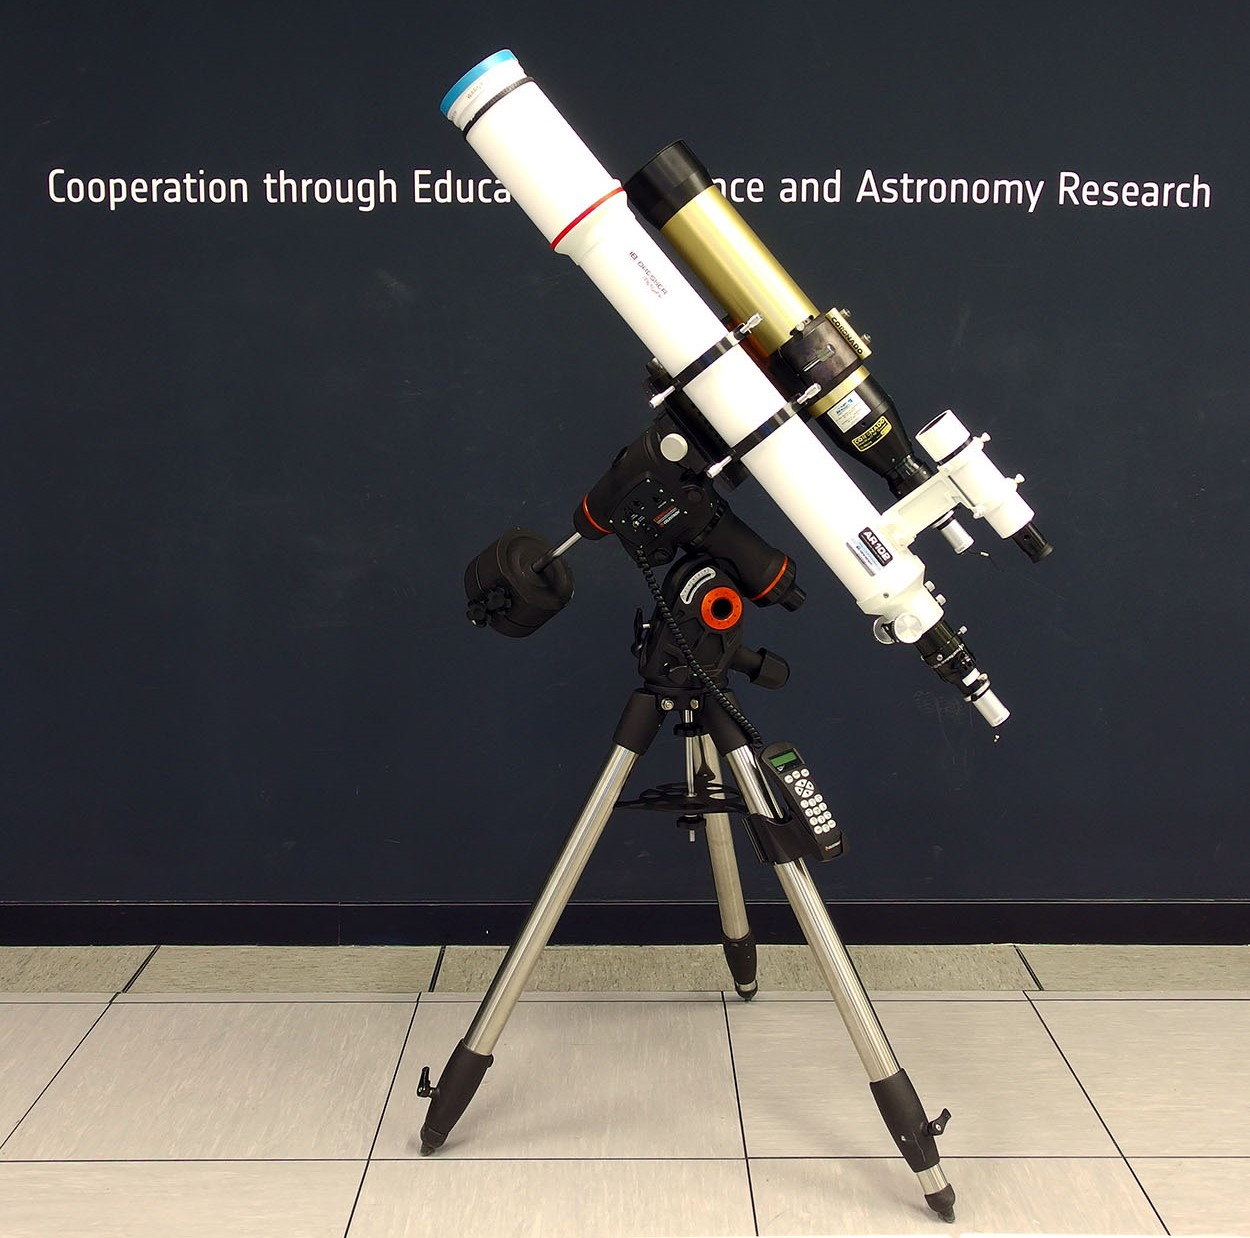
\includegraphics[height=0.4\textheight]{./pictures/solar-telescopes}
    \caption{A picture of the two telescopes}
    \label{fig:solar-telescopes}
\end{figure}
\noindent Given these differences, dedicated processing techniques are used for each telescope. Nonetheless, the preliminary steps of the two pipelines are shared, although with different parameters, and they are therefore presented together. In fact, we can logically divide the pipelines in two phases (which are treated in the next sections):
\begin{itemize}
  \item \textbf{Preliminary adjustments}, performed for both telescopes with different parameters;
  \item \textbf{Feature enhancement}, dedicated for each telescope.
\end{itemize}

\section{Preliminary Adjustments}
\noindent The first phase of the processing starts with a set of quality control checks. For each image we need to make sure that they are not corrupted or completely black, since files could be damaged during the transfer from the observatory to the servers that are allocated for the processing. Then, a second check, called cloud control, is performed to retain only the images where the Sun is perfectly visible, and discard the cloudy ones.
\bigbreak
\noindent Once it is certain that the images are up to standard, the pipeline proceeds to perform some corrections that are necessary to remove the artifacts introduced by the sensor. In fact, even the best sensors suffer from variations in the pixel sensitivity of the detector and distortions in the optical path. Luckily, is possible to account for these errors unsing two techniques that are really popular in digital photograpy: \textbf{dark-frame subtraction} and \textbf{flat-field correction}. The former tries to minimize the noise due to defective pixels and dark currents, while the latter adjusts for the relative sensitivity of pixels. The dark-frame is created by taking long exposure images in con complete darkness, or, in this case, when the lid of the telescope is on. The flat-field, instead, is generated attaching an omogeneous light source over the instrument, to measure how much each pixel reacts to it. Thus, two calibration images are used to adjust the images with the following formula:
\begin{equation}
C = \frac{(R - D)}{(F - D)}
\end{equation}
where $C$ is the corrected image, $R$ is the raw image, and $F$ and $D$ are the flat-field and the dark-frame respectively.
\bigbreak
\noindent The third subphase of the preliminary adjustments phase deals with image centering and axial tilt correction. Although, as explained in Appendix D, the telescope itself and the master control program already account for the tracking of the Sun, the limited accuracy of mechanical arms makes it necessary to use image processing techniques to align and center the solar disk to the frame. Moreover, in this case, centering the image is made easier by the fact that the shape of the object we are looking for is known and its size can be calculated with simple geometry. In fact, first, the sun can be considered a sphere, since its oblateness is neglectable; and second, the size of the appearent radius can be determined from the Sun-Earth distance. For the latter calculation it is sufficent to know the radius in pixels at one point of the orbit (we used the perihelion), and remember that the appearent size of an object depends on its distance. Therefore the radius can be calculated as:
\begin{equation}
  A_{pix} = \left( \frac{Ap_{pix}}{Ap_{rad}} \right)  \arctan{\left(\frac{r}{d}\right)}
\end{equation}
where $A_{pix}$ is the desired radius in pixels at distance $d$, $Ap_{pix}$ and $Ap_{rad}$ are respectively the appearent radius at perihelion in pixels and radians, $r$ is the absolute radius of the sun and $d$ is the Sun-Earth distance at some point of the orbit extracted from a dataset.
\bigbreak
\noindent Knowing the appearent radius for each day, it is possible to build a dynamic template of the disk, and template matching can be applied to find the center of the Sun in pixel coordinates. Also, the radius can be used to determine the size of the patch to be cropped in order to obtain an image in which the Sun is centered. The perfect alignment is achieved by rotating the resulting image by an angle that is equal to the axial tilt.

\section{Feature Enhancement}
\subsection{White-light}
\noindent For the white-light pipeline the feature enhancement phase starts with brightness correction. The brightness of the image depends on many factors, such as seeing, clouds, exposure time and gain. These factors also affect the depth of the intensity gap of sunspots. We desire to be able to account for different conditions and correct the image accordingly, while also trying to enhance sunspots.
\bigbreak
\noindent An easy solution to this problem is to use the mean intensity of the disk to adjust brightness and the standard deviation to make the depth of sunspots roughly constant. In practice, the mean is subtracted from all the pixels of the disk, then the pixel counts are scaled to achieve the desired standard deviation value and finally the new mean is added to the pixels.
\bigbreak
\noindent Depending on the puropose of the processing, whether scientific or visual, the limb darkening effect can be corrected or not. The procedure is the same as explained in section \ref{autoannotation}. Limb darkening corrections is important, in some cases, because it helps to identify those sunspots that are very close to the limb of the Sun.
\bigbreak
\noindent The processing technique that most enhances the transitions between quiet disk background, penumbra and umbra is sharpening. Since in a scientific setting it is best to retain as much information as possible, sharpening techiques that involve lossy operations like blurring were discarded. The most satisfactory performances were achieved, using second order derivative sharpening.
\bigbreak
\noindent The results of the processing can be appreciated in Figure~\ref{fig:halpha-visible}.

\subsection{H-alpha}
For what concerns the H-alpha telescope, this processing phase is very interesing, because it allows to uncover features that are not visible from the raw images. In fact, our H-alpha pipeline mainly focuses on bringing out those low intensity emissions that come from the atmosphere of the Sun. There are two phenomena that were analyzed: \textbf{prominences} and \textbf{filaments}.
\bigbreak
\noindent Both prominences and filaments are large, bright feature extending outward from the Sun's surface. They are anchored to the Sun's surface in the photosphere, but their gaseous arms reach the corona. The only difference between them is the relative position with respect to the observer. Prominences extend orthogonally to the line of sight of the observer and cross the limb of the Sun outwards. This means that they are visible as bright bands emitting on a the black background (deep space). Filaments, instead, lay inbetween the observer and the Sun, therefore they appear as dark bands on the surrounding disk.
\bigbreak
\begin{figure}[t!]
    \centering
    \captionsetup{justification=centering}
    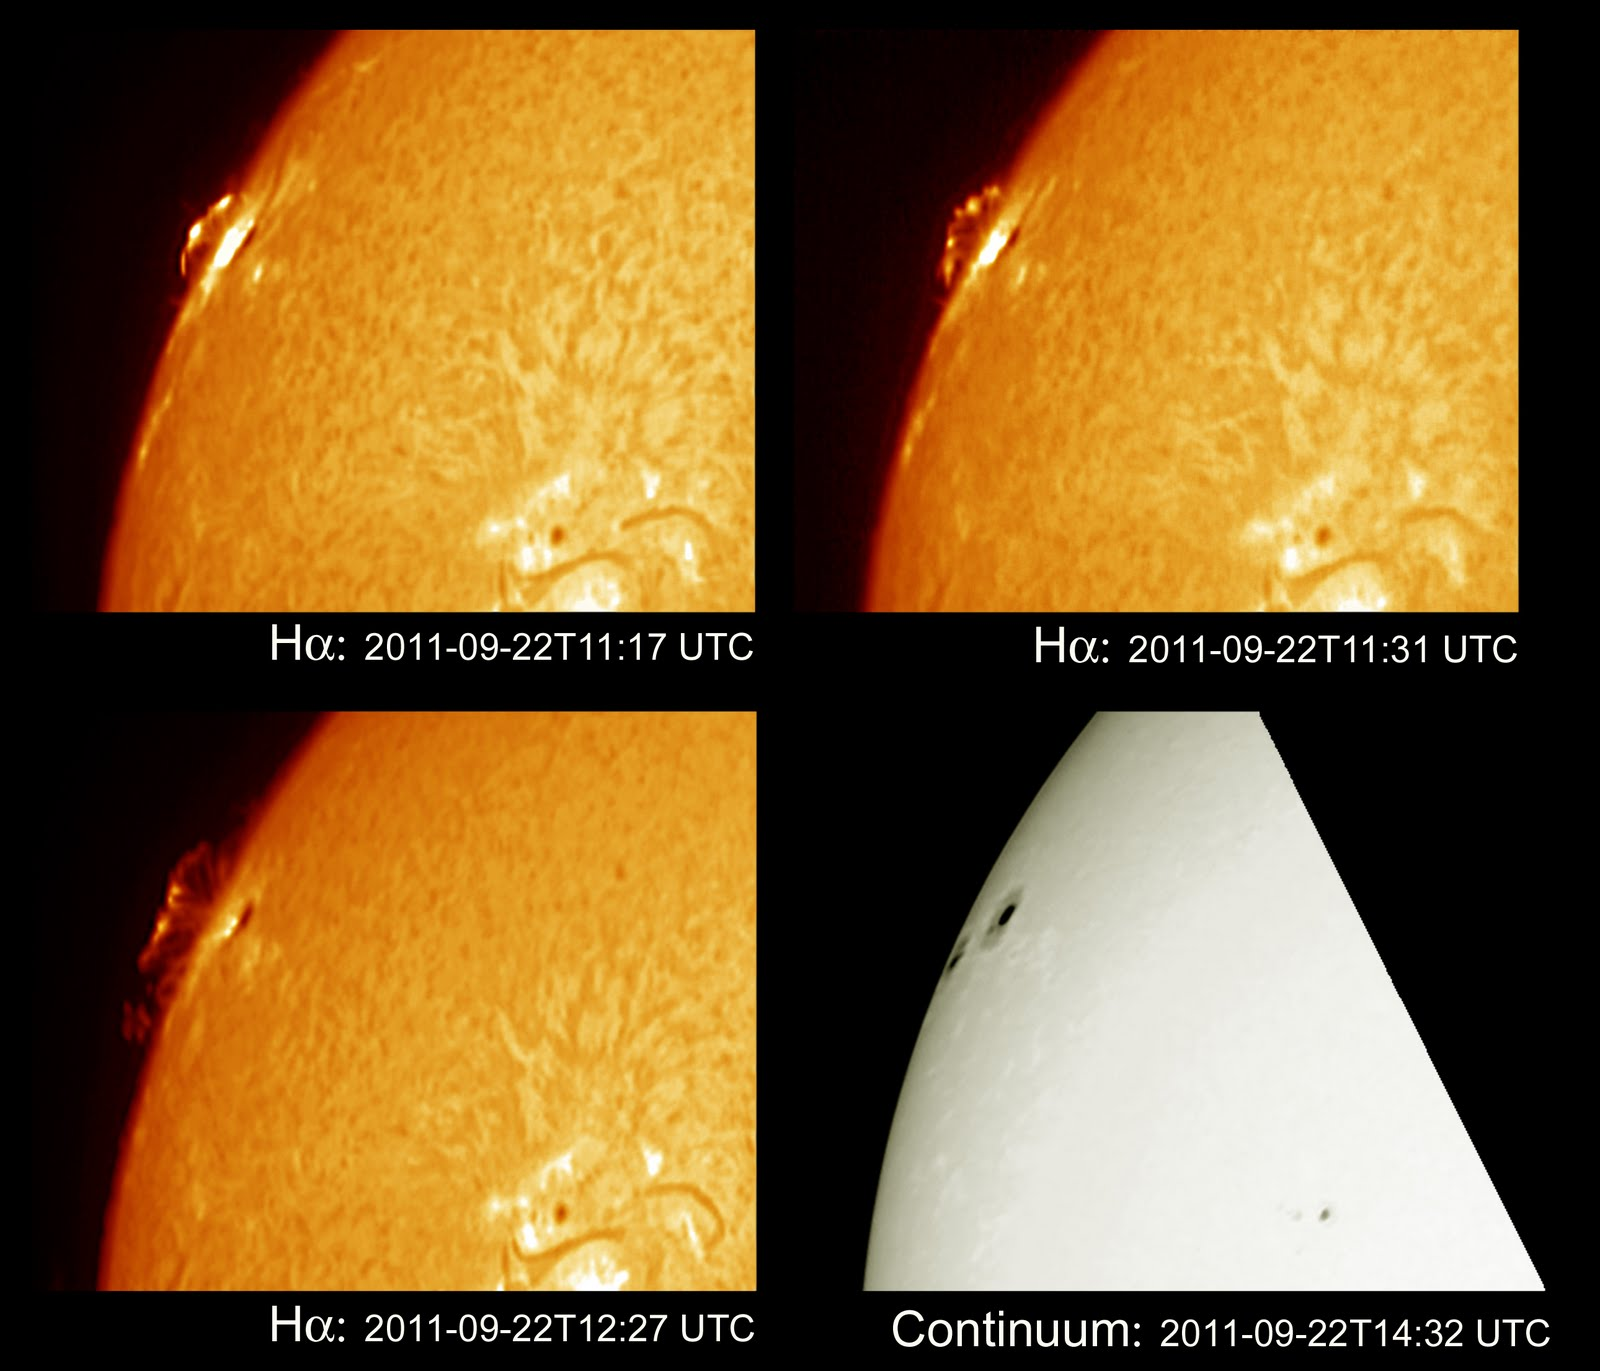
\includegraphics[width=\textwidth]{./pictures/sunsopt-flare}
    \caption{Example images taken from the Helios observatory. H-alpha (right), visible (left)}
    \label{fig:halpha-visible}
\end{figure}
\noindent The process of revealing protuberances from raw images is called off-limb emission enhancement. At the Helios observatory two such techniques were explored:
\begin{itemize}
  \item \textbf{thresholding} and \textbf{stretching}: the background is first cleaned from noise with a threshold and then the histograms stretched to increase contrast;
  \item \textbf{double exposure superposition}: two subsequent images with different exposure time are taken and then merged together. Off-limb pixel values are taken from the image with longer exposure time, while the disk is copied from the other one. Even though the time difference between the two shots is minimal, it is usually necessary to align them before performing the merger.
\end{itemize}
\bigbreak
\noindent Filaments, instead, are treated similarly to sunspots, since they both lay on the disk. The only processing that can be performed in this case is sharpening. Both gradient and laplacian sharpening have been applied for filament enhancement, with similar performance.
